\chapter{Concept}
The application should be accessible to all employees of SinnerSchrader. Due to the heterogeneity of the people’s computer setups running Windows, macOS and Linux, creating a native application supported by everyone’s system is a rather complicated task. A web application using standard technologies does not only solve this problem, but can also be used from mobile devices such as smart phones and tablets. Furthermore, there is no need to manually install and update the software so that it can be assumed that all users use the latest version of the application. This is not only a positive factor regarding the overall usability of the system, but also assures bugs and security issues are eliminated the moment a fixed version of the software is deployed. All those advantages compared to native clients and the fact that SinnerSchrader’s expertise lies in the development of web applications made the decision that this tool should be realized as such. (TODO: wording as such)



\section{Commercial Solutions}

\subsection{Skills Base}
Skills Base\footnote{http://http://www.skills-base.com/} offers the required features, but also includes a large number of functionality SinnerSchrader does not need and ist not willing to use. This includes assessments, the categorization of skills and a role model for advanced access rights configuration.
The search function does not provide searching for multiple skills. Furthermore, the sorting of results found cannot be customized. A central point of the application are dashboards displaying information about the most popular skills in the organisation and long term statistics.
\begin{figure}[h]
    \centering
    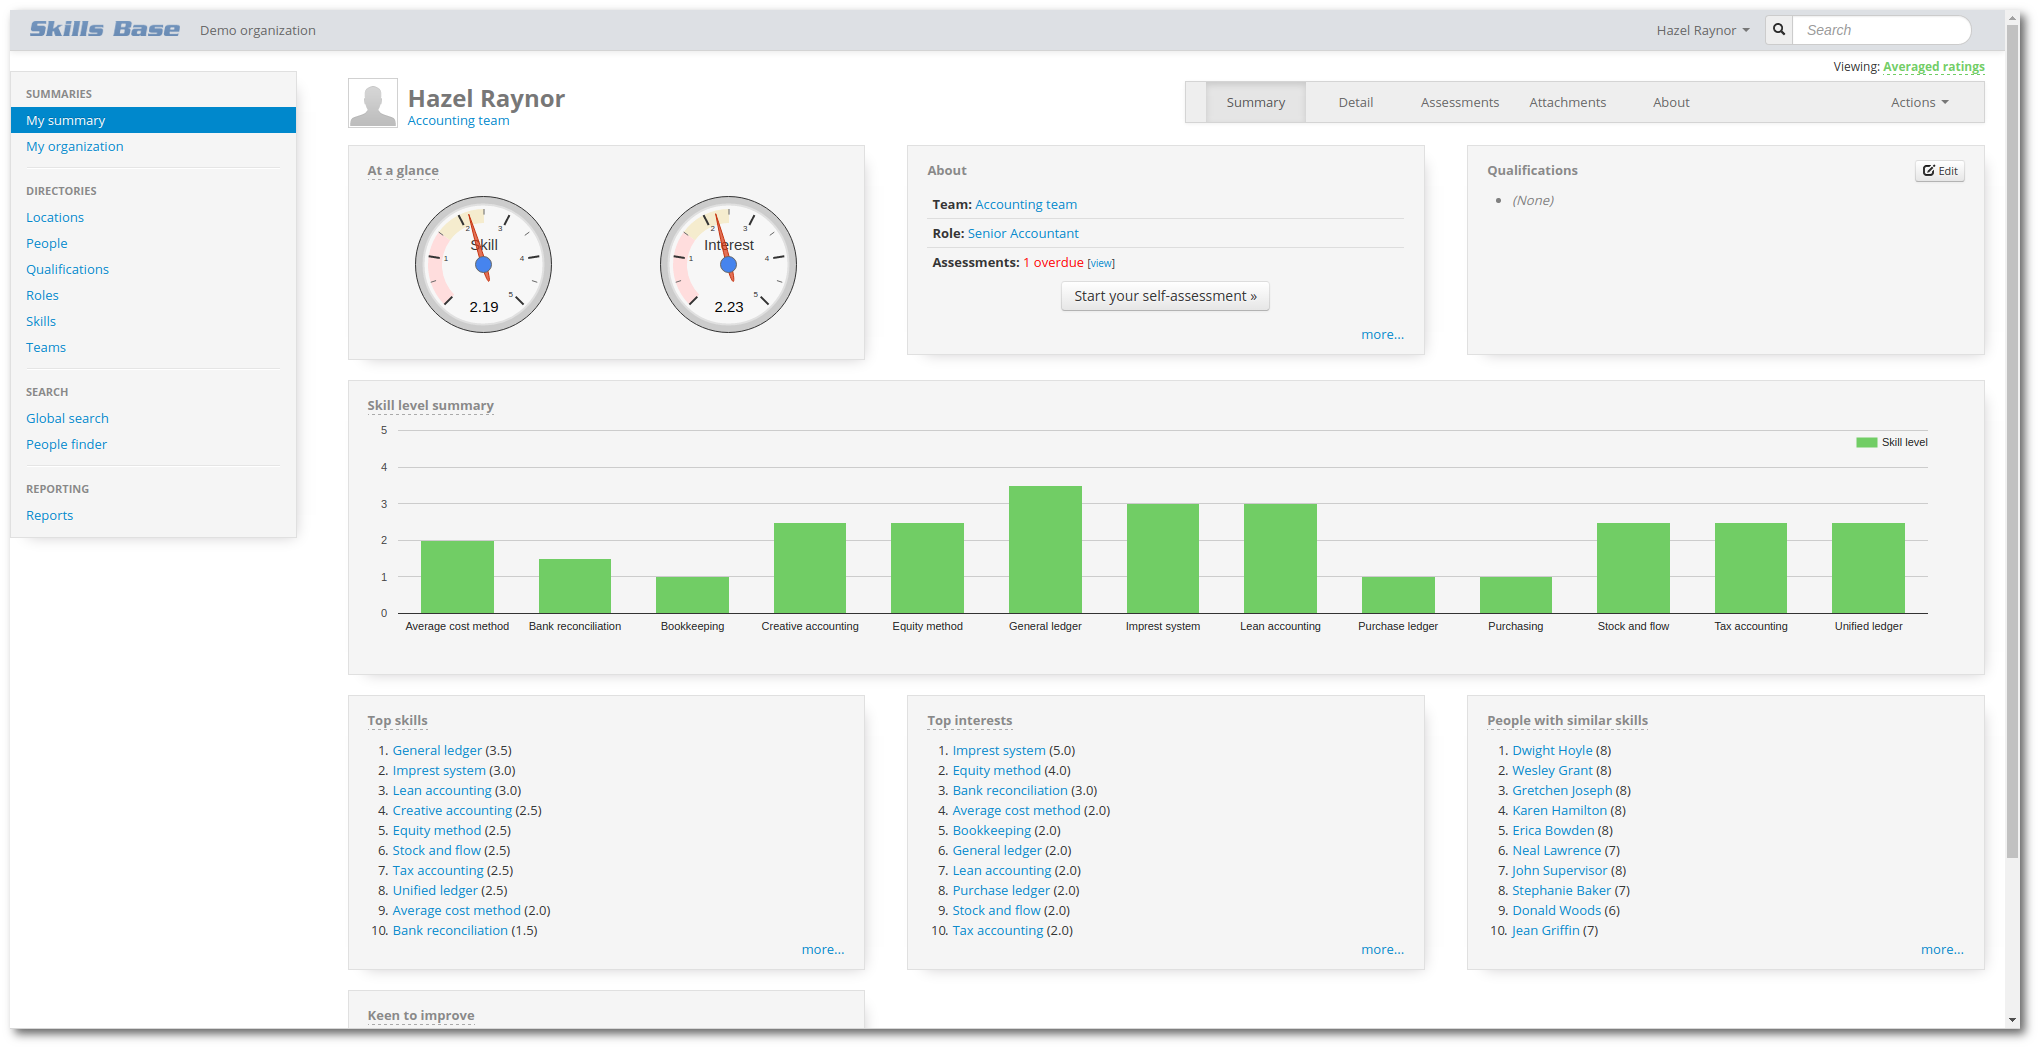
\includegraphics[width=0.8\textwidth]{images/skillsbase-dashboard.png}
    \caption{SkillsBase Dashboard}
    \label{fig:skillsbase_dashboard}
\end{figure}

\subsection{Talent Management (engage!)}
Talent Management\footnote{http://www.infoniqa.com/hr-software/skill-management} is a module for Infoniqa’s management software engage!. It offers advanced features for managers such as a powerful search function controlled via a special query language. It also includes data about the employees’ salaries, feedback protocols and certificates. It can only be used in combination with engage!, an complete human resources management solution including features like time tracking, e-learning, applicant management and payroll accounting.

\begin{figure}[h]
    \centering
    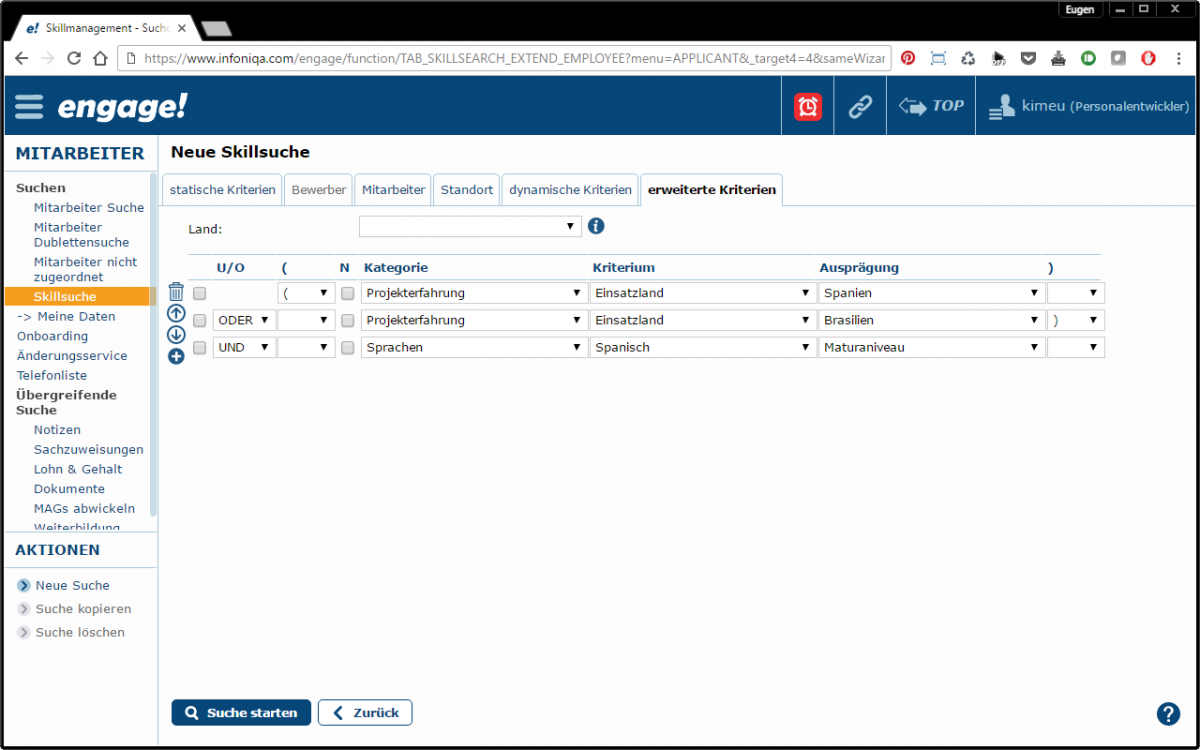
\includegraphics[width=0.8\textwidth]{images/talent_management_-_skillmanagement_-_skillsuche.png}
    \caption{Talent Management Search}
    \label{fig:talent_management}
\end{figure}

\subsection{SkillsDB Pro}
SkillsDB Pro\footnote{http://www.skillsdbpro.com} is an application designed to serve as a database in an organization providing an overview about every person’s own skills and and trainings only to themselves and their manager. The search function is capable of searching for multiple skills combined with different logical operators which enables users to enter very sophisticated queries.
Not only can users provide information about their skills, but managers can also do this with the limitation that no employee can see their manager’s rating about themselves.
Furthermore, only managers can search for persons. Taking into consideration that SinnerSchrader needs a tool to enable everyone to find someone with a specific skillset, this is a serious disadvantage.
SkillsDB also offers features SinnerSchrader does not intent to use including, but not limited to the automatic generation of project reports based on plan succession and demands for assessments.



\section{Requirements}
\subsection{Functional Requirements}
\begin{itemize}
	\item User Profiles \\
	Anyone can see another user’s profile consisting of basic information about the user such as Name, Location, E-Mail and personal skills. Personal skills are composed of a name, a knowledge level and a will level, both on a scale from one to four.
	\item Provide/Edit skills\\
	Users can add new skills from a pool of known skills to their own profile. Already added skills can be edited and removed from the profile.
	\item Search\\
	A search function can be used to find people who have added one or more specific skills to their profile. When searching for multiple skills, only persons matching all of them will will be displayed.
	\begin{itemize}
		\item Ranking\\
			By default, the search results order should be defined by a score aggregating the individuals knowledge and will levels. Employees willing to enhance their knowledge about a searched skill should be preferred to others having the same knowledge but a lower will.
		\item Sorting\\
			The user should be able to sort the search results not only by said score,
			but also solely by knowledge and will level.
	\end{itemize}
	\item Management of known skills\\
	New skills can be added to the set of known skills in the application. Existing skills can be edited and removed. Users personal skills are automatically updated when a skill has been edited so that the integrity of the user profiles is maintained at all times.
\end{itemize}



\subsection{Non Functional Requirements}
TODO: Klären und formulieren
\begin{itemize}
	\item Desktop/Devices
	\item Browsers
	\item Scalability
	\item Load/Response Times
\end{itemize}

\subsection{Revisiting Commercial Solutions}
(TODO: Featurematrix aufstellen)
As shown in (TODO: verweis auf matrix), none of the analyzed softwares (TODO verweis) offers all features required, but all of them include various functions SinnerSchrader does not intend to use, which brings undesired complexity into the applications.
One of the most critical features, sorting the search results by best match, is not offered by any of the commercial solutions.
Furthermore, all those systems differentiate between employees and their supervisors and thus restrain transparency. Instead of a solution for monitoring employees and rating them, we want a tool for everyone to find another person who offers the skills needed to solve a concrete problem.



\section{Visual Concept \& Wireframes}
The application should be as simple as possible and usable for everyone, in order to provide an efficient and fast tool. Thus, it will be designed as a single page application based around a people search that provides a way to input the skills needed and returns all persons offering said skills. After entering a search, the user can select any of the found colleagues and view their personal profile showing extended information like contact details, more skills the user did not search for, and the employee's location. This profile will also include links to directly contact the inspected person via Email or Google Hangouts(TODO: footnote). Unlike the considered commercial solutions, this tool will not include features like creating statistics, assessments, applicant management, or any dashboard other than the basic search view.
Furthermore, there will not be any different roles with different access rights for employees and their managers, since this application is meant to be a tool enhancing collaboration, not supervision.
\begin{figure}[h]
    \centering
    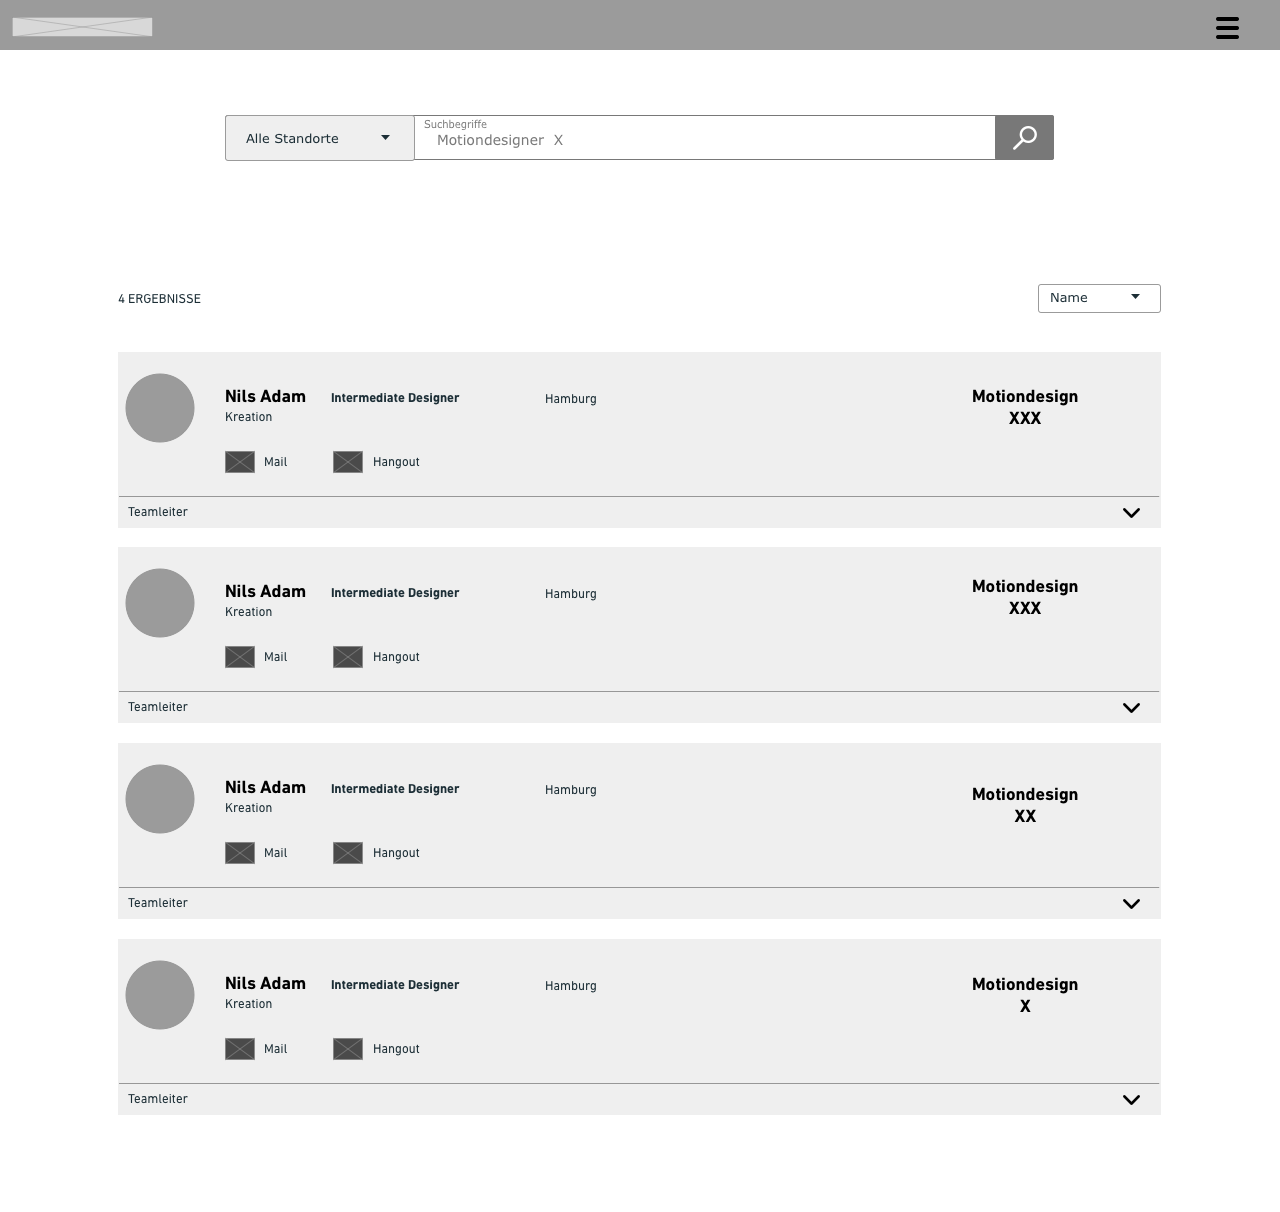
\includegraphics[width=0.8\textwidth]{images/wireframe.png}
    \caption{Wireframe}
    \label{fig:wireframe}
\end{figure}

TODO: Put UML/BPMN here

\section{Matching Algorithm}
